\chapter*{LAMPIRAN}

\section*{Kode Program}
\subsection*{Program Untuk Memeriksa MAC Address Pada ESP32}
% Program 3.1 
\begin{lstlisting}[
    language=Arduino,
    caption={Program Untuk Memeriksa MAC Address Pada ESP32},
    label={lst:CekMAC}
]
#include <BluetoothSerial.h>
BluetoothSerial SerialBT;

void setup() {
  Serial.begin(115200);
  SerialBT.begin("ESP32_Haris"); // Bluetooth device name
  delay(1000);  // Give some time for the Bluetooth module to initialize
}

void loop() {
  // Get the ESP32 Bluetooth address
  uint8_t esp32Address[6];
  esp_efuse_mac_get_default(esp32Address);

  // Print the address in a readable format
  Serial.printf("ESP32 Bluetooth Address: %02X:%02X:%02X:%02X:%02X:%02X\n",
                esp32Address[0], esp32Address[1], esp32Address[2],
                esp32Address[3], esp32Address[4], esp32Address[5]);
}
    
\end{lstlisting}

\subsection*{Program Untuk Menerima Data String Melalui Bluetooth Pada ESP32}

% Program 3.2
\begin{lstlisting}[
    language=Arduino,
    caption={Program Untuk Menerima Data String Melalui Bluetooth Pada ESP32},
    label={lst:ReceivedBluetooth}
]
#include <BluetoothSerial.h>
BluetoothSerial SerialBT;

int maxspeed;

void setup(){
  Serial.begin(115200);
  SerialBT.begin("ESP32_Haris");
}

void loop(){
  if (SerialBT.available()){
    String receivedData = SerialBT.readStringUntil('\n');

    String arah = receivedData.substring(0, receivedData.indexOf(','));
    String kecepatan = receivedData.substring(receivedData.indexOf(',') + 1);

    maxspeed = kecepatan.toInt();

    Serial.print("Arah : ");
    Serial.println(arah);
    Serial.print("Kecepatan : ");
    Serial.println(kecepatan);
    SerialBT.println("1");

    if(maxspeed < 20){
      Serial.println("TRUE");
    }
    else{
      Serial.println("FALSE");
    }
  }
}
    
\end{lstlisting}

\subsection*{Program Untuk Menerima Data JSON Melalui Bluetooth Pada ESP32}

% Program 3.3
\begin{lstlisting}[
    language=Arduino,
    caption={Program Untuk Menerima Data JSON Melalui Bluetooth Pada ESP32},
    label={lst:ReceivedBluetoothJSON}
]
#include <BluetoothSerial.h>
#include <ArduinoJson.h>

BluetoothSerial SerialBT;

void setup() {
  Serial.begin(115200);
  SerialBT.begin("ESP32_Haris");
}

void loop() {
  if (SerialBT.available()) {
    // Read the incoming data
    String json_data = SerialBT.readStringUntil('\n');

    // Deserialize the JSON
    DynamicJsonDocument doc(1024);
    DeserializationError error = deserializeJson(doc, json_data);

    if (error) {
      Serial.println("Failed to parse JSON");
    } else {
      // Extract values from JSON
      const char* arah = doc["arah"];
      const char* kecepatan = doc["kecepatan"];

      // Perform actions based on the received data
      Serial.print("Received Arah: ");
      Serial.println(arah);
      Serial.print("Received Kecepatan: ");
      Serial.println(kecepatan);
    }
  }
}
    
\end{lstlisting}

\subsection*{Program Untuk Menerima Data String Melalui \emph{Access Point} WiFi Pada ESP32}


% Program 3.4
\begin{lstlisting}[
    language=Arduino,
    caption={Program Untuk Menerima Data String Melalui \emph{Access Point} WiFi Pada ESP32},
    label={lst:ReceivedWiFi}
]
#include <WiFi.h>
#include <Arduino.h>

int maxspeed;

const char* ssid = "Haris-Access-Point";
const char* password = "123456789";

WiFiServer server(80);

void setup(){
  Serial.begin(115200);


  // Connect to Wi-Fi network with SSID and password
  Serial.print("Setting AP Access Point");
  // Remove the password parameter, if you want the AP (Access Point) to be open
  WiFi.softAP(ssid, password);
 
  IPAddress IP = WiFi.softAPIP();
  Serial.print("ESP32 AP IP Address : ");
  Serial.println(IP);

  // Start the server
  server.begin();
}

void loop(){
    // Check if a client has connected
  WiFiClient client = server.available();

  if (client) {
    //Serial.println("New client connected");
    
    // Read the data from the client
    while (client.connected()) {
      if (client.available()) {
    
        String receivedData = client.readStringUntil('\n');

        String arah = receivedData.substring(0, receivedData.indexOf(','));
        String kecepatan = receivedData.substring(receivedData.indexOf(',') + 1);

        maxspeed = kecepatan.toInt();

        Serial.print("Arah : ");
        Serial.println(arah);
        Serial.print("Kecepatan : ");
        Serial.println(kecepatan);

        if(maxspeed < 20){
          Serial.println("TRUE");
        }
        else{
          Serial.println("FALSE");
        }

      }
    }

    client.stop();

  }
}
\end{lstlisting}

\subsection*{Program Untuk Menerima Data JSON Melalui \emph{Access Point} WiFi Pada ESP32}

% Program 3.5
\begin{lstlisting}[
    language=Arduino,
    caption={Program Untuk Menerima Data JSON Melalui Access Point WiFi Pada ESP32},
    label={lst:ReceivedWiFiJSON}
]
#include <WiFi.h>
#include <Arduino.h>
#include <ArduinoJson.h>

int maxspeed;

const char* ssid = "B300-Access-Point";
const char* password = "123456789";

WiFiServer server(80);

void setup(){
  Serial.begin(115200);


  // Connect to Wi-Fi network with SSID and password
  Serial.print("Setting AP (Access Point)");
  // Remove the password parameter, if you want the AP (Access Point) to be open
  WiFi.softAP(ssid, password);
 
  IPAddress IP = WiFi.softAPIP();
  Serial.print("ESP32 AP IP Address : ");
  Serial.println(IP);

  // Start the server
  server.begin();
}

void loop(){
    // Check if a client has connected
  WiFiClient client = server.available();

  if (client) {
    //Serial.println("New client connected");
    
    // Read the data from the client
    while (client.connected()) {
      if (client.available()) {
    
        String json_data = client.readStringUntil('\n');

        DynamicJsonDocument doc(1024);
        DeserializationError error = deserializeJson(doc, json_data);

        if(error){
          Serial.println("Failed to parse JSON");
        }
        else{
          const char* arah = doc["arah"];
          int kecepatan = doc["kecepatan"];

          Serial.print("Received Arah : ");
          Serial.print(arah);
          Serial.print("   Received Kecepatan : ");
          Serial.println(kecepatan);
        }
      }
    }

    client.stop();

  }
}
\end{lstlisting}

\subsection*{Program Untuk Menguji Rangkaian Kontrol ESP32}
% Program 3.6
\begin{lstlisting}[
    language=Arduino,
    caption={Program Untuk Menguji Rangkaian Kontrol Pada ESP32},
    label={lst:MotorTest}
]
#include <Arduino.h>

//Motor Kiri
#define pwmpin1 5
#define dir1  18
#define dir2  19

//Motor kanan
#define pwmpin2 25
#define dir3 32
#define dir4 33

#define pwmChannel1  0
#define pwmChannel2  1
#define freq  15000
#define res  8

int PWM1_DutyCycle = 0;
int maxspeed = 127;


void setup() {
  // put your setup code here, to run once:
  
  pinMode(dir1,OUTPUT);
  pinMode(dir2,OUTPUT);
  pinMode(dir3,OUTPUT);
  pinMode(dir4,OUTPUT);
  //pinMode(pwmpin,OUTPUT);

  ledcSetup(pwmChannel1, freq, res);
  ledcSetup(pwmChannel2, freq, res);

  ledcAttachPin(pwmpin1, pwmChannel1);
  ledcAttachPin(pwmpin2, pwmChannel2);

  //ledcWrite(pwmChannel, 127);
}

void loop() {
  // put your main code here, to run repeatedly:

//MAJU
  //SOFTSTART
  while(PWM1_DutyCycle < maxspeed)
  {
    digitalWrite(dir1, HIGH);
    digitalWrite(dir2, LOW);
    digitalWrite(dir3, HIGH);
    digitalWrite(dir4, LOW);
    ledcWrite(pwmChannel1, PWM1_DutyCycle++);
    ledcWrite(pwmChannel2, PWM1_DutyCycle++);
    delay(10);
  }
  delay(5000);
  
  //SOFTSTOP
  while(PWM1_DutyCycle > 0)
  {
    digitalWrite(dir1, HIGH);
    digitalWrite(dir2, LOW);
    digitalWrite(dir3, HIGH);
    digitalWrite(dir4, LOW);
    ledcWrite(pwmChannel1, PWM1_DutyCycle--);
    ledcWrite(pwmChannel2, PWM1_DutyCycle--);
    delay(10);

  }
  delay(1000);

//MUNDUR
  while(PWM1_DutyCycle < maxspeed)
  {
    digitalWrite(dir1, LOW);
    digitalWrite(dir2, HIGH);
    digitalWrite(dir3, LOW);
    digitalWrite(dir4, HIGH);
    ledcWrite(pwmChannel1, PWM1_DutyCycle++);
    ledcWrite(pwmChannel2, PWM1_DutyCycle++);
    delay(10);
  }
  delay(5000);
  
  //SOFTSTOP
  while(PWM1_DutyCycle > 0)
  {
    digitalWrite(dir1, LOW);
    digitalWrite(dir2, HIGH);
    digitalWrite(dir3, LOW);
    digitalWrite(dir4, HIGH);
    ledcWrite(pwmChannel1, PWM1_DutyCycle--);
    ledcWrite(pwmChannel2, PWM1_DutyCycle--);
    delay(10);

  }
  delay(1000);

//BELOK KANAN
 while(PWM1_DutyCycle < maxspeed)
  {
    digitalWrite(dir1, HIGH);
    digitalWrite(dir2, LOW);
    digitalWrite(dir3, LOW);
    digitalWrite(dir4, LOW);
    ledcWrite(pwmChannel1, PWM1_DutyCycle++);
    ledcWrite(pwmChannel2, PWM1_DutyCycle++);
    delay(10);
  }
  delay(5000);
  
  //SOFTSTOP
  while(PWM1_DutyCycle > 0)
  {
    digitalWrite(dir1, HIGH);
    digitalWrite(dir2, LOW);
    digitalWrite(dir3, LOW);
    digitalWrite(dir4, LOW);
    ledcWrite(pwmChannel1, PWM1_DutyCycle--);
    ledcWrite(pwmChannel2, PWM1_DutyCycle--);
    delay(10);

  }
  delay(1000);

//BELOK KIRI
 while(PWM1_DutyCycle < maxspeed)
  {
    digitalWrite(dir1, LOW);
    digitalWrite(dir2, LOW);
    digitalWrite(dir3, HIGH);
    digitalWrite(dir4, LOW);
    ledcWrite(pwmChannel1, PWM1_DutyCycle++);
    ledcWrite(pwmChannel2, PWM1_DutyCycle++);
    delay(10);
  }
  delay(5000);
  
  //SOFTSTOP
  while(PWM1_DutyCycle > 0)
  {
    digitalWrite(dir1, LOW);
    digitalWrite(dir2, LOW);
    digitalWrite(dir3, HIGH);
    digitalWrite(dir4, LOW);
    ledcWrite(pwmChannel1, PWM1_DutyCycle--);
    ledcWrite(pwmChannel2, PWM1_DutyCycle--);
    delay(10);

  }
  delay(1000);

//STOP
 while(PWM1_DutyCycle < maxspeed)
  {
    digitalWrite(dir1, LOW);
    digitalWrite(dir2, LOW);
    digitalWrite(dir3, LOW);
    digitalWrite(dir4, LOW);
    ledcWrite(pwmChannel1, PWM1_DutyCycle++);
    ledcWrite(pwmChannel2, PWM1_DutyCycle++);
    delay(10);
  }
  delay(5000);
  
  //SOFTSTOP
  while(PWM1_DutyCycle > 0)
  {
    digitalWrite(dir1, LOW);
    digitalWrite(dir2, LOW);
    digitalWrite(dir3, LOW);
    digitalWrite(dir4, LOW);
    ledcWrite(pwmChannel1, PWM1_DutyCycle--);
    ledcWrite(pwmChannel2, PWM1_DutyCycle--);
    delay(10);

  }
  delay(1000);
}
\end{lstlisting}

\subsection*{Program Kontrol Motor Kursi Roda Melalui Bluetooth}

\begin{lstlisting}[
    language=Arduino,
    caption={Program Kontrol Motor Kursi Roda Melalui Bluetooth},
    label={lst:MotorBluetooth}
  ]
  #include <BluetoothSerial.h>
  #include <Arduino.h>
  
  //Motor Kiri
  #define pwmpin1 5
  #define dir1 18
  #define dir2 19
  
  //Motor kanan
  #define pwmpin2 25
  #define dir3 32
  #define dir4 33
  
  //STATE Motor
  int stdir[4];
  
  #define pwmChannel1 0
  #define pwmChannel2 1
  #define freq 15000
  #define res 8
  
  int PWM1_DutyCycle = 0;
  int maxspeed = 0;
  int turnspeed = 0;
  
  BluetoothSerial SerialBT;
  
  void setup() {
    Serial.begin(115200);
    SerialBT.begin("ESP32_Haris");
  
    pinMode(dir1, OUTPUT);
    pinMode(dir2, OUTPUT);
    pinMode(dir3, OUTPUT);
    pinMode(dir4, OUTPUT);
  
    ledcSetup(pwmChannel1, freq, res);
    ledcSetup(pwmChannel2, freq, res);
  
    ledcAttachPin(pwmpin1, pwmChannel1);
    ledcAttachPin(pwmpin2, pwmChannel2);
  }
  
  void loop() {
    if (SerialBT.available()) {
      String receivedData = SerialBT.readStringUntil('\n');
  
      String arah = receivedData.substring(0, receivedData.indexOf(','));
      String kecepatan = receivedData.substring(receivedData.indexOf(',') + 1);
  
      maxspeed = kecepatan.toInt();
      turnspeed = maxspeed / 2;
  
      Serial.print("Arah : ");
      Serial.println(arah);
      Serial.print("Kecepatan : ");
      Serial.println(kecepatan);
  
      if (arah == "A") {
        while (PWM1_DutyCycle <= turnspeed) {
          stdir[0] = LOW;
          stdir[1] = LOW;
          stdir[2] = HIGH;
          stdir[3] = LOW;
  
          digitalWrite(dir1, stdir[0]);
          digitalWrite(dir2, stdir[1]);
          digitalWrite(dir3, stdir[2]);
          digitalWrite(dir4, stdir[3]);
          ledcWrite(pwmChannel1, PWM1_DutyCycle++);
          ledcWrite(pwmChannel2, PWM1_DutyCycle++);
          delay(10);
        }
  
      } else if (arah == "B") {
        while (PWM1_DutyCycle <= maxspeed) {
          stdir[0] = HIGH;
          stdir[1] = LOW;
          stdir[2] = HIGH;
          stdir[3] = LOW;
  
          digitalWrite(dir1, stdir[0]);
          digitalWrite(dir2, stdir[1]);
          digitalWrite(dir3, stdir[2]);
          digitalWrite(dir4, stdir[3]);
          ledcWrite(pwmChannel1, PWM1_DutyCycle++);
          ledcWrite(pwmChannel2, PWM1_DutyCycle++);
          delay(10);
        }
  
      } else if (arah == "C") {
        while (PWM1_DutyCycle >= 0) {
  
          digitalWrite(dir1, stdir[0]);
          digitalWrite(dir2, stdir[1]);
          digitalWrite(dir3, stdir[2]);
          digitalWrite(dir4, stdir[3]);
          ledcWrite(pwmChannel1, PWM1_DutyCycle--);
          ledcWrite(pwmChannel2, PWM1_DutyCycle--);
          delay(10);
        }
      } else if (arah == "D") {
        while (PWM1_DutyCycle <= turnspeed) {
          stdir[0] = LOW;
          stdir[1] = HIGH;
          stdir[2] = LOW;
          stdir[3] = HIGH;
  
          digitalWrite(dir1, stdir[0]);
          digitalWrite(dir2, stdir[1]);
          digitalWrite(dir3, stdir[2]);
          digitalWrite(dir4, stdir[3]);
          ledcWrite(pwmChannel1, PWM1_DutyCycle++);
          ledcWrite(pwmChannel2, PWM1_DutyCycle++);
          delay(10);
        }
  
      } else if (arah == "E") {
        while (PWM1_DutyCycle <= turnspeed) {
          stdir[0] = HIGH;
          stdir[1] = LOW;
          stdir[2] = LOW;
          stdir[3] = LOW;
  
          digitalWrite(dir1, stdir[0]);
          digitalWrite(dir2, stdir[1]);
          digitalWrite(dir3, stdir[2]);
          digitalWrite(dir4, stdir[3]);
          ledcWrite(pwmChannel1, PWM1_DutyCycle++);
          ledcWrite(pwmChannel2, PWM1_DutyCycle++);
          delay(10);
        }
  
      }
    }
  }  
  \end{lstlisting}

\subsection*{Program Kontrol Motor Kursi Roda Melalui \emph{Access Point} WiFi}

\begin{lstlisting}[
    language=Arduino,
    caption={Program Kontrol Motor Kursi Roda Melalui \emph{Access Point} WiFi},
    label={lst:MotorWiFiAP}
  ]
  #include <WiFi.h>
  #include <Arduino.h>
  
  //WiFi Configuration
  const char* ssid = "Haris-Access-Point";
  const char* password = "123456789";
  
  WiFiServer server(80);
  
  //Motor Kiri
  #define pwmpin1 5
  #define dir1 18
  #define dir2 19
  
  //Motor kanan
  #define pwmpin2 25
  #define dir3 32
  #define dir4 33
  
  //STATE Motor
  int stdir[4];
  
  #define pwmChannel1 0
  #define pwmChannel2 1
  #define freq 15000
  #define res 8
  
  int PWM1_DutyCycle = 0;
  int maxspeed = 70;
  int turnspeed = 35;
  
  void setup() {
    Serial.begin(115200);
    Serial.print("Setting AP (Access Point) ...");
    WiFi.softAP(ssid, password);
  
    IPAddress IP = WiFi.softAPIP();
    Serial.print("ESP32 AP IP Address : ");
    Serial.println(IP);
  
    server.begin();
  
    pinMode(dir1, OUTPUT);
    pinMode(dir2, OUTPUT);
    pinMode(dir3, OUTPUT);
    pinMode(dir4, OUTPUT);
  
    ledcSetup(pwmChannel1, freq, res);
    ledcSetup(pwmChannel2, freq, res);
  
    ledcAttachPin(pwmpin1, pwmChannel1);
    ledcAttachPin(pwmpin2, pwmChannel2);
  }
  
  void loop() {
    WiFiClient client = server.available();
    if(client){
      while(client.connected()){
        if(client.available()){
  
          String arah = client.readStringUntil('\n');
          Serial.print("Arah : ");
          Serial.println(arah);
  
          if(arah == "A"){
            while(PWM1_DutyCycle <= turnspeed){
              stdir[0] = LOW;
              stdir[1] = LOW;
              stdir[2] = HIGH;
              stdir[3] = LOW;
  
              digitalWrite(dir1, stdir[0]);
              digitalWrite(dir2, stdir[1]);
              digitalWrite(dir3, stdir[2]);
              digitalWrite(dir4, stdir[3]);
              ledcWrite(pwmChannel1, PWM1_DutyCycle++);
              ledcWrite(pwmChannel2, PWM1_DutyCycle++);
              delay(10);
            }
          }
          else if(arah == "B"){
            while(PWM1_DutyCycle <= maxspeed){
              stdir[0] = HIGH;
              stdir[1] = LOW;
              stdir[2] = HIGH;
              stdir[3] = LOW;
  
              digitalWrite(dir1, stdir[0]);
              digitalWrite(dir2, stdir[1]);
              digitalWrite(dir3, stdir[2]);
              digitalWrite(dir4, stdir[3]);
              ledcWrite(pwmChannel1, PWM1_DutyCycle++);
              ledcWrite(pwmChannel2, PWM1_DutyCycle++);
              delay(10);
            }
          }
          else if(arah == "C"){
            while(PWM1_DutyCycle >= 0){
              digitalWrite(dir1, stdir[0]);
              digitalWrite(dir2, stdir[1]);
              digitalWrite(dir3, stdir[2]);
              digitalWrite(dir4, stdir[3]);
              ledcWrite(pwmChannel1, PWM1_DutyCycle--);
              ledcWrite(pwmChannel2, PWM1_DutyCycle--);
              delay(10);
            }
          }
          else if(arah == "D"){
            while(PWM1_DutyCycle <= turnspeed){
              stdir[0] = LOW;
              stdir[1] = HIGH;
              stdir[2] = LOW;
              stdir[3] = HIGH;
  
              digitalWrite(dir1, stdir[0]);
              digitalWrite(dir2, stdir[1]);
              digitalWrite(dir3, stdir[2]);
              digitalWrite(dir4, stdir[3]);
              ledcWrite(pwmChannel1, PWM1_DutyCycle++);
              ledcWrite(pwmChannel2, PWM1_DutyCycle++);
              delay(10);
            }
          }
          else if(arah == "E"){
            while(PWM1_DutyCycle <= turnspeed){
              stdir[0] = HIGH;
              stdir[1] = LOW;
              stdir[2] = LOW;
              stdir[3] = LOW;
  
              digitalWrite(dir1, stdir[0]);
              digitalWrite(dir2, stdir[1]);
              digitalWrite(dir3, stdir[2]);
              digitalWrite(dir4, stdir[3]);
              ledcWrite(pwmChannel1, PWM1_DutyCycle++);
              ledcWrite(pwmChannel2, PWM1_DutyCycle++);
              delay(10);
            }
          }
        }
      }
    }
  }  
  \end{lstlisting}

\subsection*{Program Untuk Mengirim Data String Melalui Bluetooth}

% Program 3.7
\begin{lstlisting}[
    language=Python,
    caption={Program Untuk Mengirim Data String Melalui Bluetooth},
    label={lst:SendBluetooth}
]
import bluetooth
import random
import datetime
import time

# Cari perangkat Bluetooth
nearby_devices = bluetooth.discover_devices()

# Ambil alamat MAC dari ESP32 (pastikan sudah dipasangkan sebelumnya)
esp32_address = "C0:49:EF:E7:BD:EA"  # Ganti dengan alamat MAC ESP32 yang sesuai

# Lakukan koneksi
sock = bluetooth.BluetoothSocket(bluetooth.RFCOMM)
sock.connect((esp32_address, 1))

arah = random.choice('ABCDE')
kecepatan = random.choice('OPQRSTUVW')
pesan = f"{arah},{kecepatan}"
sock.send(pesan)

date = datetime.datetime.now()
print(f"{date} -> {pesan}")

i = 0

# Terima data
while True:
    data = sock.recv(8)
    flag = data.decode("utf-8")
    #print("Received:", flag)
    
    if flag == '1':
        arah = random.choice('ABCDE')
        kecepatan = random.choice('OPQRSTUVW')
        pesan = f"{arah},{kecepatan}"
        i = i + 1
        
        if arah == 'q' or i == 10:
            break
        
        sock.send(pesan)
        date = datetime.datetime.now()
        print(f"{date} -> {pesan}")
        
# Tutup koneksi
sock.close()


\end{lstlisting}

\subsection*{Program Untuk Mengirim Data String Melalui WiFi}

\begin{lstlisting}[
    language=Python,
    caption={Program Untuk Mengirim Data String Melalui WiFi},
    label={lst:SendWiFiAP}
  ]
  import socket
  import time
  import datetime
  
  host = "192.168.4.1" # Set to ESP32 Access Point IP Address
  port = 80
  
  # Create a socket connection
  with socket.socket(socket.AF_INET, socket.SOCK_STREAM) as s:
      # Connect to the ESP32 server
      s.connect((host, port))
      
      while True:
          # Send two data values
          arah = input("Enter arah : ")
          kecepatan = input("Enter kecepatan : ")
          message = f"{arah},{kecepatan}"
          date = datetime.datetime.now()
          print(date)
      
          if arah == "q" or kecepatan == "q":
              break
      
          s.send(message.encode('utf-8'))
          
  s.close()
  
\end{lstlisting}

\subsection*{Program Untuk Mengirim Data JSON Melalui Bluetooth}

\begin{lstlisting}[
    language=Python,
    caption={Program Untuk Mengirim Data JSON Melalui Bluetooth},
    label={lst:SendBluetoothJSON}
]
import bluetooth
import json

# ESP32 Bluetooth address
esp32_address = "EC:62:60:9B:E4:92"  # Replace with your ESP32's Bluetooth address

# Create a Bluetooth socket
sock = bluetooth.BluetoothSocket(bluetooth.RFCOMM)

# Connect to the ESP32
sock.connect((esp32_address, 1))

while True:
    # Get keyboard input for two values
    arah = input("Masukkan Arah: ")
    kecepatan = input("Masukkan Kecepatan: ")
    
    # Create a JSON object
    json_data = {"arah": arah, "kecepatan": kecepatan}

    # Serialize the JSON data
    json_string = json.dumps(json_data)
    
    if arah == "q" or kecepatan == "q":
        break

    # Send the serialized JSON over Bluetooth
    sock.send(json_string)

# Close the Bluetooth socket
sock.close()

\end{lstlisting}

\subsection*{Program Untuk Mengirim Data JSON Melalui WiFi}

\begin{lstlisting}[
    language=Python,
    caption={Program Untuk Mengirim Data JSON Melalui WiFi},
    label={lst:SendWiFiJSON}
  ]
  import socket
  import time
  import json
  import datetime
  
  host = "192.168.4.1" # Set to ESP32 Access Point IP Address
  port = 80
  
  # Create a socket connection
  with socket.socket(socket.AF_INET, socket.SOCK_STREAM) as s:
      # Connect to the ESP32 server
      s.connect((host, port))
      
      while True:
          arah = input("Masukkan Arah: ")
          kecepatan = input("Masukkan Kecepatan: ")
          
          json_data = {"arah": arah, "kecepatan": kecepatan}
          date = datetime.datetime.now()
          
          if arah == q or kecepatan == q:
              break
          else:
              json_string = json.dumps(json_data)
              s.send(json_string.encode('utf-8'))
              print(f"{date} -> {json_data}")
  
  s.close()
\end{lstlisting}

\subsection*{Pengujian Kestabilan Motor Kursi Roda}
\begin{figure} [ht] \centering
  % Nama dari file gambar yang diinputkan
  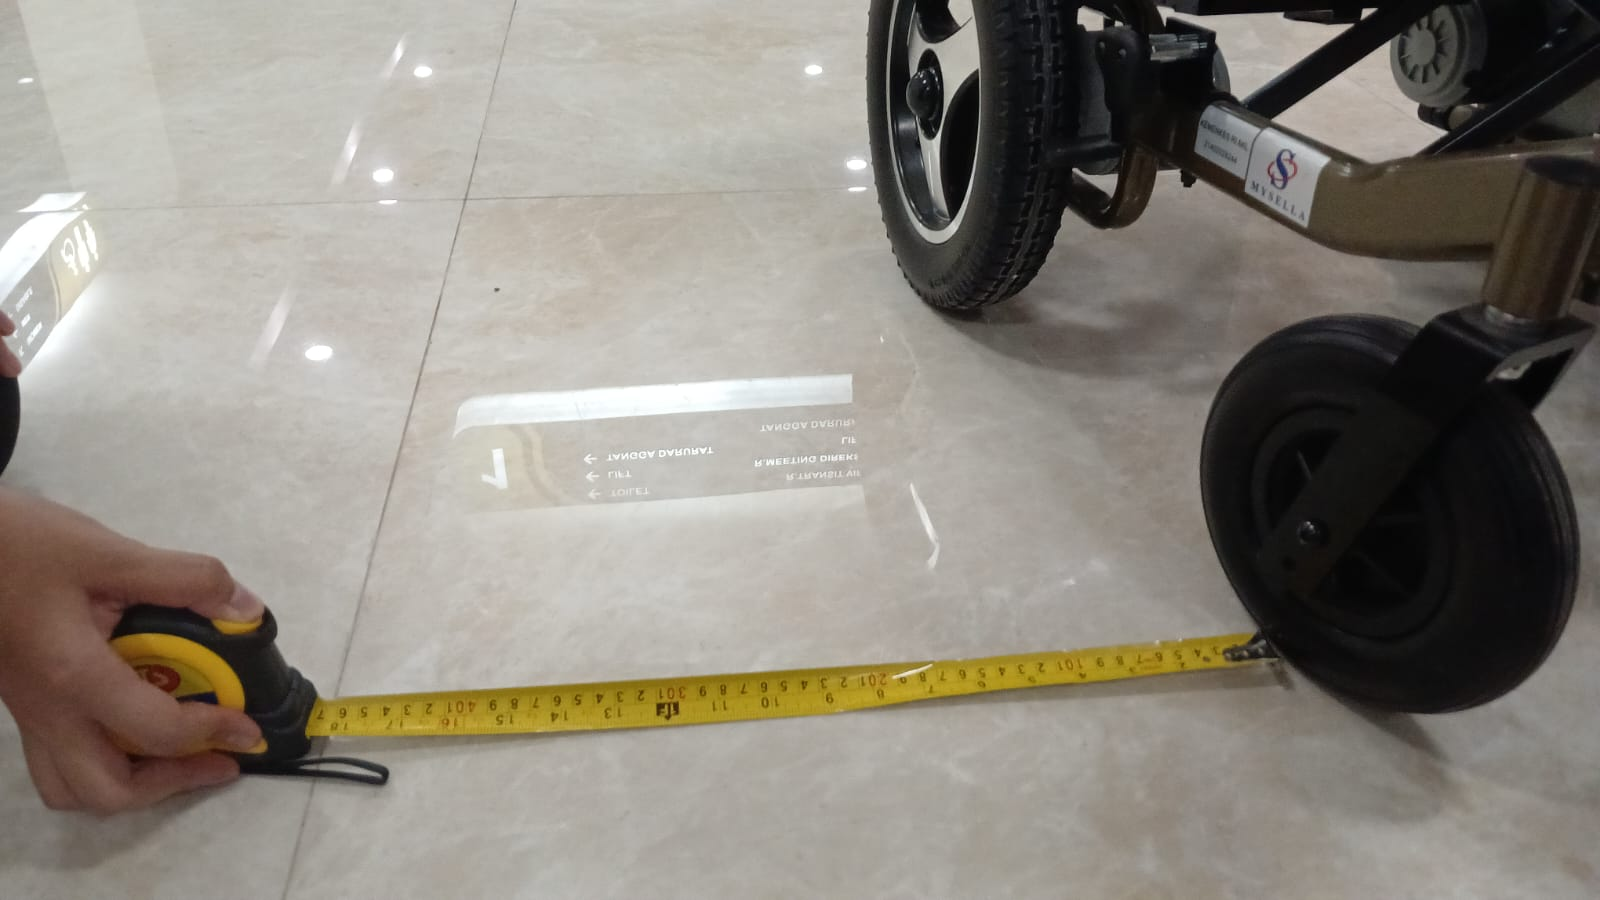
\includegraphics[scale=0.28]{gambar/lampiran/Pengujian Kestabilan.jpg}
  % Keterangan gambar yang diinputkan
  \caption{Dokumentasi Perhitungan Jarak Penyimpangan}
  % Label referensi dari gambar yang diinputkan
  \label{fig:DokumentasiJarakPenyimpangan}
\end{figure}